\chapter{Diseño del experimento}

Utilizando los estudios de \cite{Fontanella2000} y  \cite{Vidal1964} pudimos obtener las reglas definidas en el capítulo anterior. Recordemos que éstas describen la diferencia entre los dos grupos. En este capítulo proponemos realizar un experimento para extraer la información fonética de los mismos. La idea será realizar una serie de actividades donde el hablante sea grabado y que esas actividades hagan hincapié en estas diferencias descriptas. A continuación vamos a describir el experimento en más detalle.

\section{Elección de las frases}

El acento se potencia cuando se realiza habla espontánea. Utilizando este concepto intentamos que el hablante diga las frases de la forma más natural posible. Es por ello que elegimos como actividad pronunciar frases popularmente conocidas. Si el hablante conoce la frase y la utiliza con frecuencia entonces es más fácil que su pronunciación sea espontánea. Con esta idea vamos a cubrir las reglas 2 al 6. 

Recordemos que en el capítulo anterior la regla 1 nos decía que había una diferencia en la duración de la sílaba previa a la acentuada: para hablantes de Córdoba esta duración es más corta que para hablantes de Buenos Aires. La sílaba acentuada varía según que tipo de palabra se refiere. No es lo mismo utilizar una palabra aguda que una esdrújula en esta regla. Para cubrir esta regla utilizamos un esquema de frases con una estructura fija pero que varía sus palabras según su entonación. Este esquema se llama AMPER \cite{amper2004,amper} y lo veremos más en detalle en la sección \ref{cap:amper}.

Entonces los esquemas van a ser: 

\begin{itemize}
  \item \textbf{Frases utilizando esquema AMPER que cubre cada tipo de acentuación:} Estas corresponden a la regla 1 que hace énfasis en la longitud de la sílaba anterior a la acentuada. Utilizamos este esquema para cubrir todo tipo de acentuación.
  \item \textbf{Frases comunes que tratan de cubrir la espontaneidad:} Estas frases van a cubrir las reglas 2 a 6. Estas tienen que ver con la duración y la pronunciación de distintos fonemas. Utilizar frases comunes favorece la espontaneidad.
\end{itemize}

A continuación vemos las reglas en sus dos conjuntos.

\subsection{Frases utilizando esquema AMPER} \label{cap:amper}

%AMPER-ARGENTINA: VARIABILIDAD RÍTMICA EN DOS CORPUS 
%Jorge A. Gurlekian LIS - Conicet y UBA jag@fmed.uba.ar 
%Reina Yanagida LIS y Universidad Municipal de Estudios Extranjeros de Kobe, Japón reinay@hotmail.co.jp 
%Mónica Noemí Trípodi LIS – UBA monica906@hotmail.com 
%Guillermo Toledo Conicet y Universidad Laval, Canadá guillermo.toledo@sympatico.ca 

Utilizamos este esquema para analizar todas las variantes posibles de la regla 1. Recordemos que esa regla nos dice que hay que estirar la sílaba anterior a la acentuada. Esta regla define comúnmente la tonada cordobeza y puede aparecer de varias formas según su acentuación. 

Para tomar este esquema nos basamos en el trabajo de variabilidad rítmica en dos corpus \cite{amper} que utilizan un esquema similar. Este trabajo estudió los acentos del español argentino utilizando un esquema de frase fija y intercambiando palabras para analizar todos sus casos. En nuestro trabajo tenemos un problema similar por ello lo tomamos como referencia.

El esquema AMPER utilizado en este trabajo es: 
\begin{center}
\textit{Sujeto+`` salió ’’+Adjetivo} 
\end{center}

\begin{itemize}
	\item Objeto puede ser \textit{``El canapé’’, ``El repollo’’, ``El espárrago’’}.
	\item Adjetivo puede ser \textit{``espectacular’’, ``delicioso’’, ``riquísimo’’}.
\end{itemize}

Utilizamos estas palabras ya que cubren los tres tipos de acentuación: aguda, grave y esdrújula. 

Por ejemplo: \textit{``El canapé salió delicioso’’}. Canapé tiene acento en la última sílaba, es una palabra aguda, mientras que delicioso es grave. En este ejemplo podemos analizar la sílaba anterior a la acentuada de los dos grupos estudiados, Córdoba y Buenos Aires. Armamos las combinaciones para obtener muchas variantes de dónde se encuentra el acento. De esta forma estudiamos en detalle la regla 1. Todas las combinaciones se pueden ver en el tabla \ref{fig21table}.

%\begin{figure}[h!]
%    \centerline{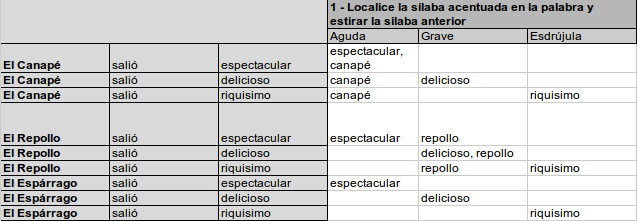
\includegraphics[width=1\textwidth]{reglas_AMPER} }
%    \caption{Frases AMPER}
%    \label{fig21}
%\end{figure}

\scriptsize
\begin{longtable}{| p{0.15\textwidth} | p{0.08\textwidth} | p{0.10\textwidth} || p{0.12\textwidth} | p{0.12\textwidth} | p{0.12\textwidth} |} 
	\hline
	%\multicolumn{6}{| p{0.9\textwidth} |} {\textbf{1 - Localice la sílaba acentuada en la palabra y estirar la sílaba anterior}} \\ \hline
	\multicolumn{3}{| p{0.45\textwidth} ||}{Frase} & \textbf{Aguda} & \textbf{Grave} & \textbf{Esdrújula} \\ \hline 
	\textit{El canapé} & \textit{salió} & \textit{espectacular} & espectacular, canapé & & \\ \hline
	\textit{El canapé} & \textit{salió} & \textit{delicioso} & canapé & delicioso & \\ \hline
	\textit{El canapé} & \textit{salió} & \textit{riquísimo} & canapé & & riquísimo \\ \hline
	\textit{El repollo} & \textit{salió} & \textit{espectacular} & espectacular & repollo & \\ \hline
	\textit{El repollo} & \textit{salió} & \textit{delicioso} &  & repollo, delicioso & \\ \hline	
	\textit{El repollo} & \textit{salió} & \textit{riquísimo} & & repollo & riquísimo \\ \hline
	\textit{El espárrago} & \textit{salió} & \textit{espectacular} & espectacular & & \\ \hline
	\textit{El espárrago} & \textit{salió} & \textit{delicioso} & & delicioso & \\ \hline
	\textit{El espárrago} & \textit{salió} & \textit{riquísimo} & & & riquísimo \\ \hline	
		
	\caption{Frases AMPER} 
	\label{fig21table}
\end{longtable}

\normalsize
\subsection{Frases comunes}

Como afirmamos antes, se utilizaron frases comunes para poder obtener los acentos de cada grupo de forma natural. Se pensó que si se graba una frase popular, el hablante al estar acostumbrado a decirla no iba a poder evitar impregnarle su acento. Todas las frases utilizadas se pueden ver en la tabla \ref{fig22tabla}.

Algo interesante es que una misma frase puede extraer atributos para varias reglas. Por ejemplo: la frase \textit{`En la pelea se conoce al soldado, sólo en la victoria se conoce al caballero’} extrae atributos para las reglas 4 y 5. La palabra \textit{`victoria’} cubre la regla 4 que nos propone medir la duración de la \textit{/c/} antes de la \textit{/t/}. Sucede igual con la palabra \textit{`caballero’} para la regla 5: el fonema \textit{/ll/} se pasa a \textit{/i/} cambiando su duración y sonido. En la Tabla \ref{fig22tabla} podemos ver que la cantidad de frases utilizadas con respecto a sus reglas es despareja. Hay más frases para la regla 2 que para las demás. Más adelante veremos como impacta esto en las frases que vamos a pedir grabar.


\subsubsection{Orden de las frases}

Ya definimos cuáles van a ser las frases, ahora debemos definir qué frases y en qué orden se deben decir durante el experimento. Diremos que una frase cubre una determinada regla si esta la satisface. Sucede que el orden que utilicemos va a ser crucial para obtener muestras: no es lo mismo empezar por una frase que sólo cubre una sola regla que varias reglas al mismo tiempo. Si elegimos primero las frases que cubren varias reglas a la vez, en una sola grabación podremos obtener más cubrimiento de reglas. Entonces, en caso de poder, elegimos frases que cubran más de una regla. 

¿Por qué quisiéramos cubrir más reglas en una misma frase? Más adelante veremos que una frase grabada que cubre una regla aportará información sobre el hablante de esa regla en particular. Si una frase cubre varias reglas estaríamos obteniendo más información que si esa frase cubre una sola regla, en ambas opciones utilizamos sólo una grabación. Por eso es importante maximizar el cubrimiento de las frases por cada grabación.  

El orden de las frases sigue el siguiente algoritmo:

\lstset{ %
	language=C++,                % choose the language of the code
	basicstyle=\footnotesize,       % the size of the fonts that are used for the code
	numbers=left,                   % where to put the line-numbers
	numberstyle=\footnotesize,      % the size of the fonts that are used for the line-numbers
	stepnumber=1,                   % the step between two line-numbers. If it is 1 each line will be numbered
	numbersep=5pt,                  % how far the line-numbers are from the code
	backgroundcolor=\color{white},  % choose the background color. You must add \usepackage{color}
	showspaces=false,               % show spaces adding particular underscores
	showstringspaces=false,         % underline spaces within strings
	showtabs=false,                 % show tabs within strings adding particular underscores
	frame=single,           % adds a frame around the code
	tabsize=2,          % sets default tabsize to 2 spaces
	captionpos=b,           % sets the caption-position to bottom
	breaklines=true,        % sets automatic line breaking
	breakatwhitespace=false,    % sets if automatic breaks should only happen at whitespace
	escapeinside={\%*}{*)},          % if you want to add a comment within your code
	morekeywords={OrdenDeFrasesConocidas, String, ObtenerReglaConMenorPorcentaje, ObtenerLaFraseMasPonderada, Repetir, veces, Si, agregar, Recorrer, Devolver, y, RecalcularPorcentajes, esta, en, Mientras, Input, Output},
}
\begin{lstlisting}
OrdenDeFrasesConocidas:
Input: Frases (conj. de String)
Output: listaFrases (lista de String)
listaFrases = {}
DicPct <- Diccionario de porcentajes de cada regla
Mientras Frases != {}:
	regla <- DicPct.ObtenerReglaConMenorPorcentaje()
	frase <- Frases.ObtenerLaFraseMasPonderada(regla)
	listaFrases.agregar(frase)
	DicPct.RecalcularPorcentajes()
Devolver listaFrases
\end{lstlisting}


%\begin{figure}[h!]
%    \centerline{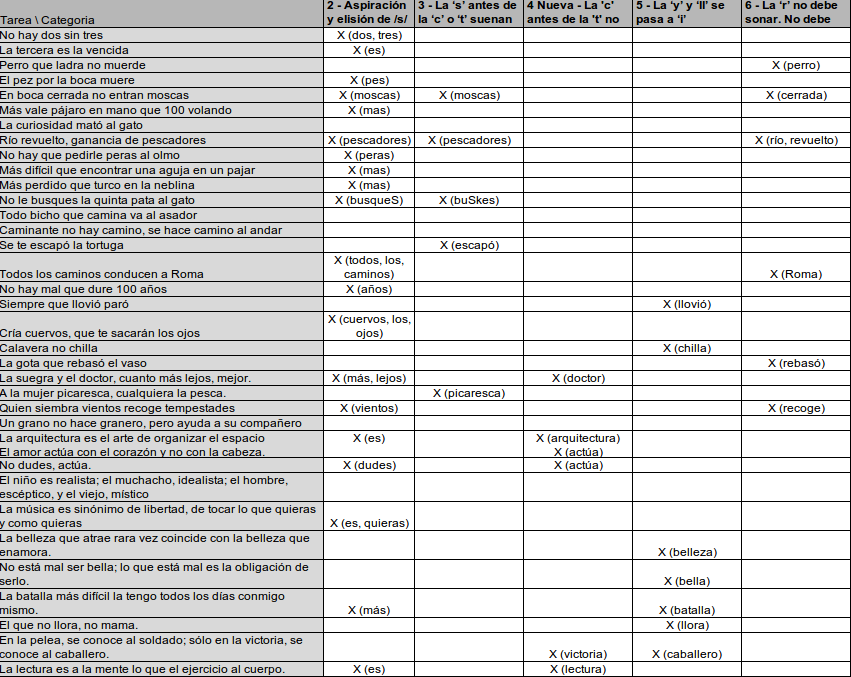
\includegraphics[width=1\textwidth]{frases_inf} }
%    \caption{Frases conocidas}
%    \label{fig22}
%\end{figure}

\newgeometry{margin=2cm} 
\begin{landscape}
\scriptsize
\begin{longtable}{| p{0.5\textwidth} || p{0.15\textwidth} | p{0.15\textwidth} | p{0.15\textwidth} | p{0.15\textwidth}| p{0.15\textwidth} | } 
	\hline
	\textbf{Frase} & \textbf{2 - Aspiración y elisión de /s/} & \textbf{3 - La 's' antes de la 'c' o 't' no suenan} & \textbf{4 - La 'c' antes de la 't' no suenan}& \textbf{5 - La 'y' y 'll' se pasa a 'i'} & \textbf{6 - La 'r' no debe sonar} \\ \hline	
	
	1 - `No hay dos sin tres' & dos, tres & & & & \\ \hline
	2 - `Más difícil que encontrar una aguja en un pajar' & más &&&& \\ \hline
	3 - `Más perdido que turco en la neblina' & más &&&&  \\ \hline
	4 - `No le busques la quinta pata al gato' & busques & busques &&&  \\ \hline
%	'Todo bicho que camina va al asador' &  \\ \hline
%	'Caminante no hay camino se hace camino al andar' &  \\ \hline
	5 - `Se te escapó la tortuga' && escapó &&&  \\ \hline
	6 - `Todos los caminos conducen a Roma' & todos, los, caminos &&&&  \\ \hline
	7 - `No hay mal que dure cien a\~nos' & a\~nos &&&& \\ \hline
	8 - `Siempre que llovió, paró' &&&& llovió & \\ \hline
	9 - `Cría cuervos que te sacaran los ojos' & cuervos, los, ojos &&&&  \\ \hline
	10 - `La tercera es la vencida' & es &&&& \\ \hline
	11 - `Calavera no chilla' &&&& chilla &  \\ \hline
	12 - `La gota que rebalsó el vaso' &&&&& rebasó \\ \hline
	13 - `La suegra y el doctor cuanto más lejos mejor' & más, lejos & doctor&&& \\ \hline
	14 - `A la mujer picaresca cualquiera la pesca' && picaresca &&&  \\ \hline
	15 - `Quien siembra vientos recoge tempestades' & vientos &&&& recoge  \\ \hline
%	'Un grano no hace granero pero ayuda a su compañero' & \\ \hline
	16 - `La arquitectura es el arte de organizar el espacio' & es && arquitectura && \\ \hline
	17 - `El amor actúa con el corazón y no con la cabeza' &&& actúa&& \\ \hline
	18 - `No dudes, actúa' &&& actúa&&  \\ \hline
%	'El niño es realista; el muchacho, idealista; el hombre, escéptico, y el viejo místico' &  \\ \hline
	19 - `Perro que ladra no muerde' &&&&& perro \\ \hline
	20 - `La musica es sinónimo de libertad, de tocar lo que quieras y cómo quieras' & es, quieras &&&& \\ \hline
	21 - `La belleza que atrae rara vez coincide con la belleza que enamora' &&&& belleza & \\ \hline
	22 - `No esta mal ser bella, lo que está mal es la obligación de serlo' &&&& bella & \\ \hline
	23 - `La batalla más difícil la tengo todos los días conmigo mismo' & más &&& batalla & \\ \hline
	24 - `El que no llora, no mama' &&&& llora & \\ \hline
	25 - `En la pelea se conoce al soldado, sólo en la victoria se conoce al caballero' &&& victoria & caballero &\\ \hline
	26 - `La lectura es a la mente lo que el ejercicio al cuerpo' & es && lectura &&  \\ \hline
	27 - `El pez por la boca muere' & pez &&&& \\ \hline
	28 - `En boca cerrada no entran moscas' & moscas & moscas &&& cerrada  \\ \hline
	29 - `Más vale pájaro en mano que cien volando' & más &&&& \\ \hline
%	'La curiosidad mató al gato' &  \\ \hline
	30 - `Río revuelto, ganancia de pescadores' & pescadores & pescadores &&& río, revuelto  \\ \hline
	31 - `No hay qué pedirle peras al olmo' & peras &&&& \\ \hline
	
	\caption{Frases conocidas} 
	\label{fig22tabla}
\end{longtable}
\end{landscape}
\restoregeometry

\normalsize

%Texto viejo primera entrega
%La idea del algoritmo es la siguiente: vamos a utilizar un contador que nos va a decir cuántas muestras tenemos por cada regla. En cada paso vamos a ver ese contador y vamos a elegir la próxima frase teniéndolo en cuenta. Esta elección la lleva a cabo la función \textit{ObtenerLaMasPonderada}. Esta se encarga de elegir la frase que haga referencia a la regla menos grabada y además que represente a más de una regla. De esa forma intentamos obtener la mayor cantidad de información posible con pocas grabaciones y ponderamos las frases que referencien a más reglas. 

La idea del algoritmo es la siguiente: vamos a contabilizar la cantidad de muestras por cada regla. Esto se realiza calculando, para cada regla, la cantidad de muestras que ya grabamos cubriendo esa regla; sobre la cantidad total de muestras que cubren esa regla. Entonces tendremos para cada regla su porcentaje de cubrimiento. Esto lo guardaremos en \textit{DicPct}.

Mientras haya frases sin ser seleccionadas para grabar, elegimos la regla que menos está cubierta. O sea, elegiremos como próxima regla a cubrir la que tenga menor porcentaje de cubrimiento. Esto se realiza llamando al método \textit{ObtenerReglaConMenorPorcentaje} del objeto \textit{DicPct}. Si hay varias con el mismo mínimo porcentaje, se elige una al azar.

Tenemos definida la próxima regla a cubrir. Debemos elegir la frase que cubra esa regla. Recordemos que hay muchas frases que cubren una determinada regla. Para definir cuál frase elegir vamos a optar por la que cubra mayor cantidad de reglas. Si hay varias frases en esta situación, elegimos una de estas al azar. Entonces no sólo aumentamos la cantidad de frases de la regla menos cubierta, sino que con esa frase cubrimos otras reglas. Esto se realiza en el método \textit{ObtenerLaFraseMásPonderada}. Para terminar, agregamos la frase elegida y recalculamos los porcentajes de cada regla en las lineas 9 y 10.

Esta idea es importante ya que llevamos al máximo la cantidad de información en cada frase y al hablante le hacemos perder menos tiempo realizando el experimento.

Podemos ver un ejemplo de este algoritmo en la tabla \ref{pasos_algo}. Este muestra los primeros 15 pasos que realiza el algoritmo en un ejemplo. Descartamos los demás pasos por simplicidad. La columna ``Tarea'' nos muestra el número de orden de la frase a grabar, ``Número de Frase'' nos indica qué frase fue la elegida para esa tarea, y las columnas ``Regla X'' muestran el porcentaje de apariciones ya grabadas de esa regla. En el primer paso todas las reglas están en 0\%, lo cual sucede porque al comienzo no se grabó ninguna frase aún.  Elegimos una frase que cumpla con la regla que tiene menor porcentaje de cubrimiento. Como todas las reglas tienen 0\% elegimos una al azar, en este ejemplo la frase 15, que cubre las reglas 2 y 6 (ver Figura \ref{fig22tabla}). Entonces el porcentaje de cubrimiento de esas reglas se incrementa. 
La frase 15 nos dice \textit{``Quien siembra vientos recoge tempestades''} y, como dijimos, cubre la regla 2 y 6. Para la regla 2 hay 26 posibles muestras en todas las frases. La frase 15 sólo aporta 1 de ellas, entonces $1/26$ nos aporta el 3\% de cubrimiento. Para la regla 6, tenemos 6 posibles muestras y esta frase nos provee sólo 1 de ellas. Su porcentaje entonces es $1/6 = 16\%$. 

El ejemplo de  la tabla \ref{pasos_algo} ilustra cómo el algoritmo, en cada paso, elige una frase que cubra la regla con menor porcentaje de cubrimiento. Por ejemplo: en la tarea 5, la regla 5 sólo tiene el 14\% de porcentaje grabado. Este cubrimiento es el menor de todos. En el próximo paso, el algoritmo elige una frase que cubra esa regla y, si es posible, que cubra otra regla más. La elegida es la frase 23 (ver \ref{fig22tabla}). Como hay pocas frases de la regla 5, al agregar esta frase ya cubrimos el 28\% de las frases de esa regla. Y además se incrementa la regla 2 al 23\%. De este modo, intentamos ir cubriendo paso a paso en forma pareja las distintas reglas.

\scriptsize
\begin{longtable}{| p{0.1\textwidth} | p{0.08\textwidth} || p{0.1\textwidth} | p{0.1\textwidth} | p{0.1\textwidth} | p{0.1\textwidth} | p{0.1\textwidth} |
		p{0.1\textwidth} |} 
	\hline
	
	\textbf{Tarea} & \textbf{Nro de Frase} & \textbf{Regla 2} & \textbf{Regla 3} & \textbf{Regla 4} & \textbf{Regla 5} & \textbf{Regla 6}   \\ \hline 	
	- & -- & 0\% & 0\% & 0\% & 0\% & 0\% \\ \hline
	1 & 15 & 3\% & 0\% & 0\% & 0\% & 16\% \\ \hline
	2 & 25 & 3\% & 0\% & 20\% & 14\% & 16\% \\ \hline
	3 & 30 & 7\% & 16\% & 16\% & 14\% & 50\% \\ \hline
	4 & 28 & 11\% & 33\% & 16\% & 14\% & 66\% \\ \hline
	5 & 13 & 19\% & 50\% & 16\% & 14\% & 66\% \\ \hline
	6 & 23 & 23\% & 50\% & 16\% & 28\% & 66\% \\ \hline
	7 & 16 & 27\% & 50\% & 33\% & 28\% & 66\% \\ \hline
	8 & 26 & 30\% & 50\% & 50\% & 28\% & 66\% \\ \hline
	9 & 8  & 30\% & 50\% & 50\% & 42\% & 66\% \\ \hline
	10 & 4  & 34\% & 66\% & 50\% & 42\% & 66\% \\ \hline
	11 & 6  & 46\% & 66\% & 50\% & 42\% & 66\% \\ \hline
	12 & 21 & 46\% & 66\% & 50\% & 57\% & 66\% \\ \hline
	13 & 9  & 57\% & 66\% & 50\% & 57\% & 66\% \\ \hline
	14 & 17 & 57\% & 66\% & 66\% & 57\% & 66\% \\ \hline
	15 & 1  & 65\% & 66\% & 66\% & 57\% & 66\% \\ \hline
	\multicolumn{7}{| p{0.78\textwidth} |}{...}	\\ \hline
	
	\caption{Pasos del algoritmo OrdenDeFrasesConocidas} 
	\label{pasos_algo}
\end{longtable}

\normalsize

Esta idea también se puede ver en la Figura \ref{figFracesTraza} que representa otro ejemplo del porcentaje de frases completadas. Teniendo en cuenta este algoritmo podemos notar que aproximadamente a partir de 10 grabaciones ya tenemos un buen porcentaje de cubrimiento. Por ejemplo, en la décima grabación la regla 4 ya tiene el 75\% de sus muestras grabadas. La regla 5 el 50\% de sus muestras ya grabadas. En este ejemplo, en la grabación número 10 ya se grabó alrededor del 40\% de la cantidad total de muestras para cada regla.


\subsection{Combinando los dos tipos de frases utilizando trazas}

Definimos frases comunes y AMPER para grabar. Ahora debemos definir cómo vamos a ir intercalando cada tipo en el experimento. Para ello definimos traza. Una traza es una lista de las frases que va a grabar un hablante en el experimento. Esta va a estar compuesta por entre 1 y 3 frases comunes extraídas del orden definido en \textit{OrdenDeFrasesConocidas}, y luego una frase del esquema de AMPER. Tanto la cantidad de frases comunes como la elección de la frase AMPER se realiza al azar. Este patrón se repite sucesivamente hasta completar todas las frases. La idea es no cansar al hablante con frases repetitivas y evitar que sepa de antemano qué frase va a tener que grabar ya que si fuera el caso, podría exagerar la entonación.

Al empezar el experimento, al hablante se le dará una traza que grabará sucesivamente en ese orden. Elegimos tener precalculadas las trazas para evitar cálculos costosos a la hora de empezar el experimento. Si no se precalcularan las trazas, deberíamos realizar los cálculos cada vez que empieza el experimento y podríamos retrasar la grabación del hablante. Es por eso que guardamos 10.000 trazas generadas. 

%\begin{figure}[h!]
%    \centerline{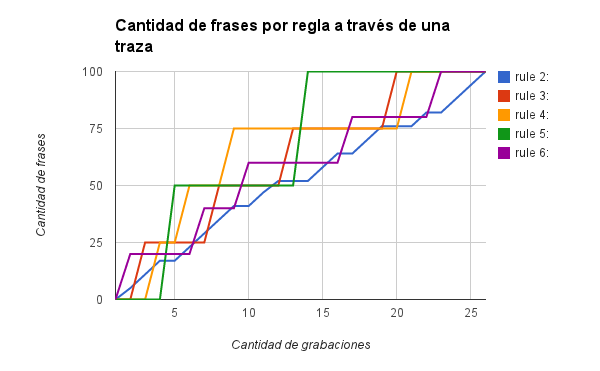
\includegraphics[width=0.9\textwidth]{cant_frases_traza_inf} }
    %\caption{Cantidad de frases por traza}
    %\label{figFracesTraza}
%\end{figure}

\begin{figure}[H]
	\centering
	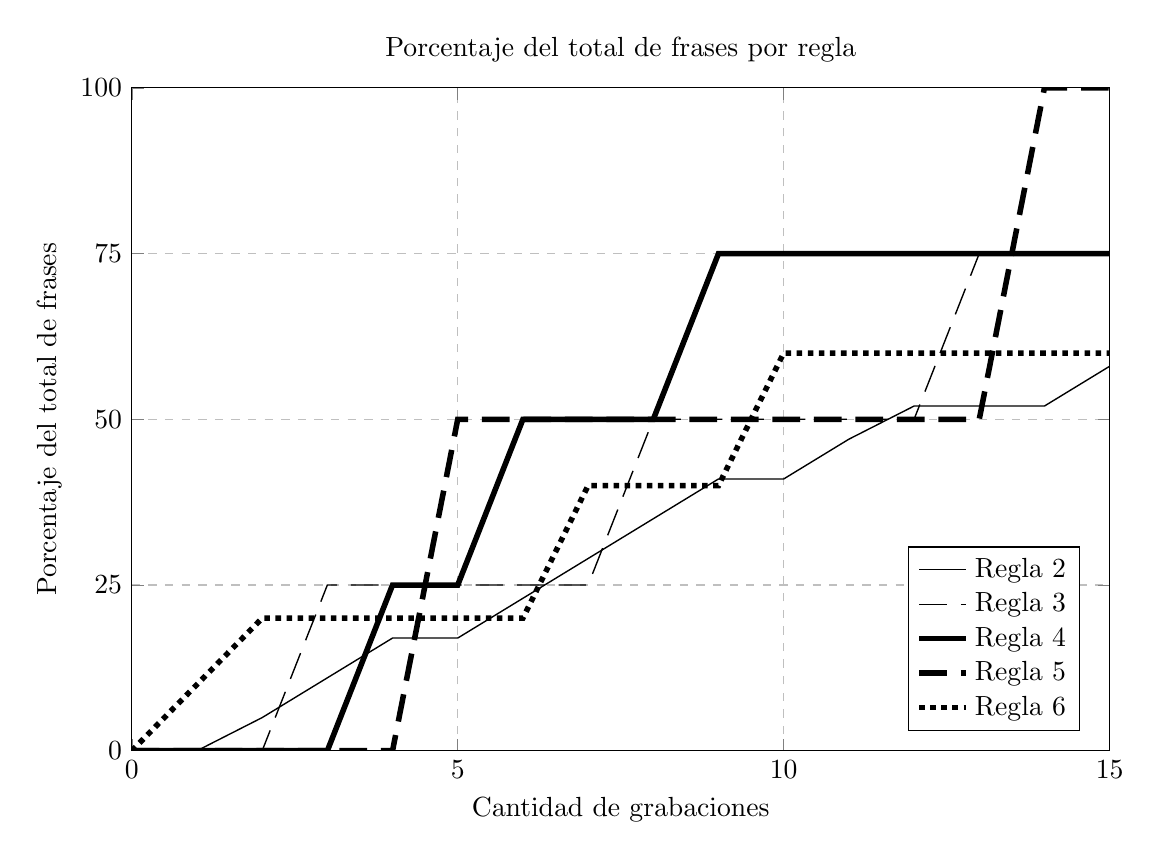
\begin{tikzpicture}
	\begin{axis}[
	width=14cm,
	height=10cm,
	title={Porcentaje del total de frases por regla},
	xlabel={Cantidad de grabaciones},
	ylabel={Porcentaje del total de frases},
	xmin=0, xmax=15,
	ymin=0, ymax=100,
	xtick={0,5,10,15,20,25,30},
	ytick={0, 25, 50, 75, 100},
	legend pos=south east,
	ymajorgrids=true,
	xmajorgrids=true,
	grid style=dashed
	] 
	
	\addplot [mark=times*, line width=0.5pt]
	coordinates {
  		(0,0)(1, 0)(2, 5)(3, 11)(4, 17)(5, 17)(6, 23)(7, 29)(8, 35)(9, 41)(10, 41)(11, 47)(12, 52)(13, 52)(14, 52)(15,58)(16, 64)(17, 64)(18, 70)(19, 76)(20, 76)(21, 76)(22, 82)(23, 82)(24, 88)(25, 94)(26, 100)
	};\addlegendentry{Regla 2};
	
	\addplot [mark=times*, dash pattern=on 10pt off 5pt, line width=0.5pt]
	coordinates {
		(0,0)(1,0)(2,0)(3,25)(4,25)(5,25)(6,25)(7,25)(8,50)(9,50)(10,50)(11,50)(12,50)(13,75)(14,75)(15,75)(16,75)(17,75)(18,75)(19,75)(20,100)(21,100)(22,100)(23,100)(24,100)(25,100)(26,100)
	};\addlegendentry{Regla 3};
	
	\addplot [mark=times*, line width=2pt] 
	coordinates {
		(0,0)(1, 0)(2, 0)(3, 0)(4, 25)(5, 25)(6, 50)(7, 50)(8, 50)(9, 75)(10, 75)(11, 75)(12, 75)(13, 75)(14, 75)(15,75)(16, 75)(17, 75)(18, 75)(19, 75)(20, 75)(21, 100)(22, 100)(23, 100)(24,100)(25,100)(26, 100)
	};\addlegendentry{Regla 4};
	
	\addplot [mark=times*, dash pattern=on 10pt off 5pt, line width=2pt]
	coordinates {
		(0,0)(4,0)(5,50)(13,50)(14,100)(26,100) 
	};\addlegendentry{Regla 5};
	
	\addplot [mark=times*, dotted, line width=2pt] 
	coordinates {
		(0,0)(2,20)(6,20)(7,40)(9,40)(10,60)(16,60)(17,80)(22,80)(23,100) 
	};\addlegendentry{Regla 6};
		
		
%%		Tarea	rule 2:	rule 3:	rule 4:	rule 5:	rule 6:
%		1	0	0	0	0	0
%		2	5	0	0	0	20
%		3	11	25	0	0	20
%		4	17	25	25	0	20
%		5	17	25	25	50	20
%		6	23	25	50	50	20
%		7	29	25	50	50	40
%		8	35	50	50	50	40
%		9	41	50	75	50	40
%		10	41	50	75	50	60
%		11	47	50	75	50	60
%		12	52	50	75	50	60
%		13	52	75	75	50	60
%		14	52	75	75	100	60
%		15	58	75	75	100	60
%		16	64	75	75	100	60
%		17	64	75	75	100	80
%		18	70	75	75	100	80
%		19	76	75	75	100	80
%		20	76	100	75	100	80
%		21	76	100	100	100	80
%		22	82	100	100	100	80
%		23	82	100	100	100	100
%		24	88	100	100	100	100
%		25	94	100	100	100	100
%		26	100	100	100	100	100
		
	\end{axis}
	\end{tikzpicture}
    \caption{Porcentaje del total de frases grabadas por cada regla}
    \label{figFracesTraza}
\end{figure}

La mínima cantidad de grabaciones que puede realizar un hablante son 5 grabaciones. Luego se le pregunta si quiere continuar grabando. Si acepta, se le agregan otras 5 grabaciones, siguiendo así sucesivamente hasta completar todas las frases a grabar de su traza. Elegimos grabar cada 5 grabaciones para que el hablante aporte el tiempo que tenga disponible y no obligarlo a grabar todas las frases. Aunque no grabe la totalidad de frases, las muestras van a servir en el experimento.

A continuación veremos cómo implementamos el sistema de grabación para soportar este experimento.
